%Chapter 2
\chapter{Overview of simulation and compressed air applications}
\label{Chap2}
\thispagestyle{empty}
\vspace{38em}
\hrulefill
\\-
\enquote*{\textit{Quote.}} - Somebody\\
\clearpage
\section{Introduction}
\section{Background on mining compressed air networks}
\subsection{Preamble}
Compressed air is used extensively in a mine in surface and underground operations. In this section, background on compressed air systems is provided through discussion of component that make up the system. 
\subsection{Compressor air network components}
\subsubsection{Compressors}
 ***  compress process inefficient ** 
\subsubsection{Pneumatic rock drills}
Drilling is mainly performed in the production areas or stopes of a mine. Drill machines are used to drill holes into the rock face. Once the holes have been drilled, explosives are then installed to break up the rock \cite{van2008development}.
\par
Compressed air is used to power pneumatic rock drills within a mine. Pneumatic rock drills run at an efficiency of 2\%. This is low when compared to alternative rock drills such as electric, oil electro-hydraulic and hydro-powered drills that run at an efficiency of between 20-31\% \cite{fraser2008saving}, \cite{vanTonder2010Masters}. 
\subsubsection{Refuge bays}
Refuge bays are installed underground in deep level mines to provide safety to miners in the event of an emergency. To satisfy the safety criteria, most mines will utilize compressed air to deliver cool air to the chamber \cite{brake1999criteria}. \cref{fig: Refuge Bay} shows an example of a compressed air inlet at an underground refuge bay. A muffler is installed to the end of the inlet air pipe to reduce noise.
\begin{figure}[h]
	\centering
	\fbox{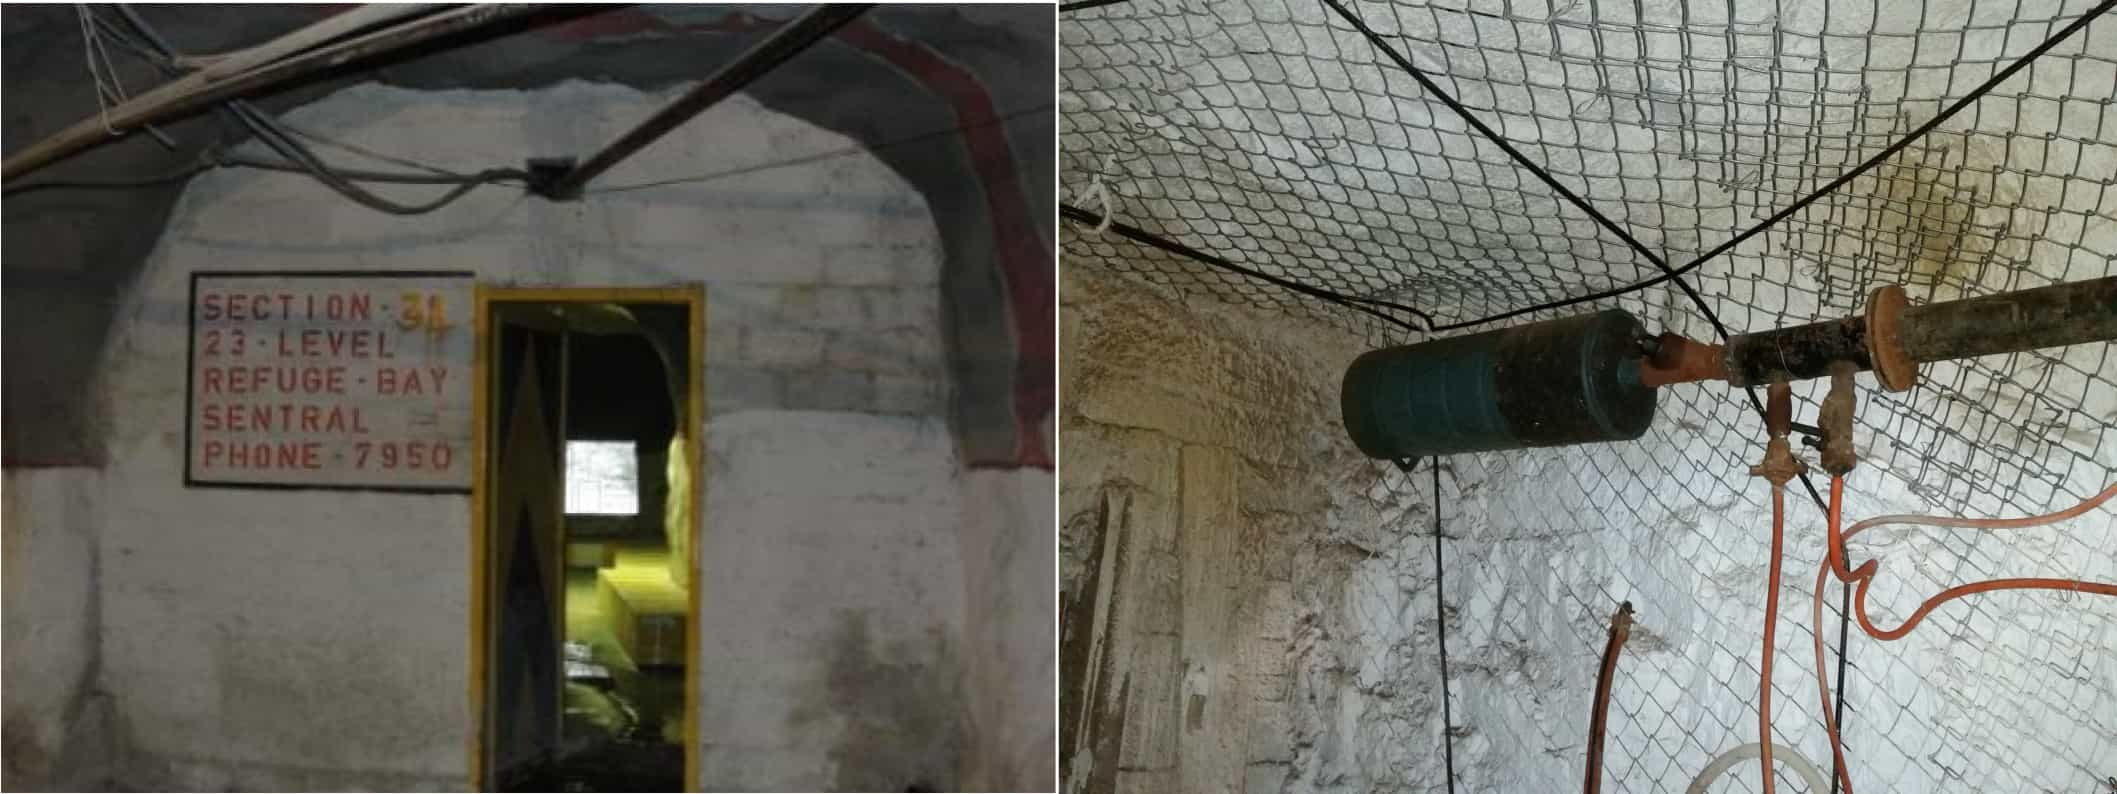
\includegraphics[width=\textwidth]{Images/1/refugebay.jpg}}
	\caption{An example of compressed air inlet in an underground refuge bay chamber of a mine.}
	\label{fig: Refuge Bay}
\end{figure}
\par The provision of 1.42 $l/s$ of air per person at a pressure between 200 and 300 \gls{kpa} is required to provide oxygen and prevent any poisonousness gas entering the refuge \cite{brake1999criteria}.\par
Airflow in the refuge bays can be controlled with a manual valve within the chamber. Often, this valve is often misused by mine workers who open the valves fully in order to cool the bay through decompression of the air.[CitationNeeded]
\subsubsection{Processing plants}
Processing plants are constructed near gold and mines. They are used when extracting metal from the ore that is obtained from the mining operation. These plants use compressed air for various systems, processes and equipment. 
\par 
To save costs, processing plants often share compressed air network with mine \cite{Marais2012PhD}. The plants use relatively low amounts of air compared to mines, however plant processes have pressure requirements that differ from the rest of the air network. If the plant is not isolated from the mine air network, compressed air optimizations on the mine can be complicated. 
\subsubsection{Other compressed air users}
Due to the availability underground, compressed air is utilised for a number of other applications. These usages include, pneumatic loaders or rock shovels, pneumatic cylinders, dam sediment agitation, cooling and ventilation and many other applications. This vast variety of of applications also leads to misuse of compressed air this leads to inefficient operation.
\subsection{Operation schedule}
On a typical mine, various operations will take place at different times of the day. Depending on the activity taking place, many mines will control the pressure to meet the requirements \cite{Kriel2014Masters},\cite{Marais2012PhD}. \cref{fig: Mining schedule} shows the schedule and pressure requirement on a typical deep level mine.\par 
As shown in the figure, the pressure requirement changes depending on the activity taking place. The drilling shift typically has the highest pressure requirement whilst blasting shift requires the lowest. Schedules and operation philosophies can differ between mines. Different operational schedules require alternative pressure requirement profiles.
\begin{figure}[h]
	\centering
	\fbox{% GNUPLOT: LaTeX picture with Postscript
\begingroup
  \makeatletter
  \providecommand\color[2][]{%
    \GenericError{(gnuplot) \space\space\space\@spaces}{%
      Package color not loaded in conjunction with
      terminal option `colourtext'%
    }{See the gnuplot documentation for explanation.%
    }{Either use 'blacktext' in gnuplot or load the package
      color.sty in LaTeX.}%
    \renewcommand\color[2][]{}%
  }%
  \providecommand\includegraphics[2][]{%
    \GenericError{(gnuplot) \space\space\space\@spaces}{%
      Package graphicx or graphics not loaded%
    }{See the gnuplot documentation for explanation.%
    }{The gnuplot epslatex terminal needs graphicx.sty or graphics.sty.}%
    \renewcommand\includegraphics[2][]{}%
  }%
  \providecommand\rotatebox[2]{#2}%
  \@ifundefined{ifGPcolor}{%
    \newif\ifGPcolor
    \GPcolortrue
  }{}%
  \@ifundefined{ifGPblacktext}{%
    \newif\ifGPblacktext
    \GPblacktextfalse
  }{}%
  % define a \g@addto@macro without @ in the name:
  \let\gplgaddtomacro\g@addto@macro
  % define empty templates for all commands taking text:
  \gdef\gplbacktext{}%
  \gdef\gplfronttext{}%
  \makeatother
  \ifGPblacktext
    % no textcolor at all
    \def\colorrgb#1{}%
    \def\colorgray#1{}%
  \else
    % gray or color?
    \ifGPcolor
      \def\colorrgb#1{\color[rgb]{#1}}%
      \def\colorgray#1{\color[gray]{#1}}%
      \expandafter\def\csname LTw\endcsname{\color{white}}%
      \expandafter\def\csname LTb\endcsname{\color{black}}%
      \expandafter\def\csname LTa\endcsname{\color{black}}%
      \expandafter\def\csname LT0\endcsname{\color[rgb]{1,0,0}}%
      \expandafter\def\csname LT1\endcsname{\color[rgb]{0,1,0}}%
      \expandafter\def\csname LT2\endcsname{\color[rgb]{0,0,1}}%
      \expandafter\def\csname LT3\endcsname{\color[rgb]{1,0,1}}%
      \expandafter\def\csname LT4\endcsname{\color[rgb]{0,1,1}}%
      \expandafter\def\csname LT5\endcsname{\color[rgb]{1,1,0}}%
      \expandafter\def\csname LT6\endcsname{\color[rgb]{0,0,0}}%
      \expandafter\def\csname LT7\endcsname{\color[rgb]{1,0.3,0}}%
      \expandafter\def\csname LT8\endcsname{\color[rgb]{0.5,0.5,0.5}}%
    \else
      % gray
      \def\colorrgb#1{\color{black}}%
      \def\colorgray#1{\color[gray]{#1}}%
      \expandafter\def\csname LTw\endcsname{\color{white}}%
      \expandafter\def\csname LTb\endcsname{\color{black}}%
      \expandafter\def\csname LTa\endcsname{\color{black}}%
      \expandafter\def\csname LT0\endcsname{\color{black}}%
      \expandafter\def\csname LT1\endcsname{\color{black}}%
      \expandafter\def\csname LT2\endcsname{\color{black}}%
      \expandafter\def\csname LT3\endcsname{\color{black}}%
      \expandafter\def\csname LT4\endcsname{\color{black}}%
      \expandafter\def\csname LT5\endcsname{\color{black}}%
      \expandafter\def\csname LT6\endcsname{\color{black}}%
      \expandafter\def\csname LT7\endcsname{\color{black}}%
      \expandafter\def\csname LT8\endcsname{\color{black}}%
    \fi
  \fi
    \setlength{\unitlength}{0.0500bp}%
    \ifx\gptboxheight\undefined%
      \newlength{\gptboxheight}%
      \newlength{\gptboxwidth}%
      \newsavebox{\gptboxtext}%
    \fi%
    \setlength{\fboxrule}{0.5pt}%
    \setlength{\fboxsep}{1pt}%
\begin{picture}(9360.00,4032.00)%
    \gplgaddtomacro\gplbacktext{%
      \colorrgb{0.00,0.00,0.00}%
      \put(814,1364){\makebox(0,0)[r]{\strut{}$400$}}%
      \colorrgb{0.00,0.00,0.00}%
      \put(814,1615){\makebox(0,0)[r]{\strut{}$420$}}%
      \colorrgb{0.00,0.00,0.00}%
      \put(814,1866){\makebox(0,0)[r]{\strut{}$440$}}%
      \colorrgb{0.00,0.00,0.00}%
      \put(814,2117){\makebox(0,0)[r]{\strut{}$460$}}%
      \colorrgb{0.00,0.00,0.00}%
      \put(814,2368){\makebox(0,0)[r]{\strut{}$480$}}%
      \colorrgb{0.00,0.00,0.00}%
      \put(814,2618){\makebox(0,0)[r]{\strut{}$500$}}%
      \colorrgb{0.00,0.00,0.00}%
      \put(814,2869){\makebox(0,0)[r]{\strut{}$520$}}%
      \colorrgb{0.00,0.00,0.00}%
      \put(814,3120){\makebox(0,0)[r]{\strut{}$540$}}%
      \colorrgb{0.00,0.00,0.00}%
      \put(814,3371){\makebox(0,0)[r]{\strut{}$560$}}%
      \colorrgb{0.00,0.00,0.00}%
      \put(946,1232){\rotatebox{-270}{\makebox(0,0)[r]{\strut{}00:00}}}%
      \colorrgb{0.00,0.00,0.00}%
      \put(1295,1232){\rotatebox{-270}{\makebox(0,0)[r]{\strut{}01:00}}}%
      \colorrgb{0.00,0.00,0.00}%
      \put(1643,1232){\rotatebox{-270}{\makebox(0,0)[r]{\strut{}02:00}}}%
      \colorrgb{0.00,0.00,0.00}%
      \put(1992,1232){\rotatebox{-270}{\makebox(0,0)[r]{\strut{}03:00}}}%
      \colorrgb{0.00,0.00,0.00}%
      \put(2340,1232){\rotatebox{-270}{\makebox(0,0)[r]{\strut{}04:00}}}%
      \colorrgb{0.00,0.00,0.00}%
      \put(2689,1232){\rotatebox{-270}{\makebox(0,0)[r]{\strut{}05:00}}}%
      \colorrgb{0.00,0.00,0.00}%
      \put(3037,1232){\rotatebox{-270}{\makebox(0,0)[r]{\strut{}06:00}}}%
      \colorrgb{0.00,0.00,0.00}%
      \put(3386,1232){\rotatebox{-270}{\makebox(0,0)[r]{\strut{}07:00}}}%
      \colorrgb{0.00,0.00,0.00}%
      \put(3734,1232){\rotatebox{-270}{\makebox(0,0)[r]{\strut{}08:00}}}%
      \colorrgb{0.00,0.00,0.00}%
      \put(4083,1232){\rotatebox{-270}{\makebox(0,0)[r]{\strut{}09:00}}}%
      \colorrgb{0.00,0.00,0.00}%
      \put(4431,1232){\rotatebox{-270}{\makebox(0,0)[r]{\strut{}10:00}}}%
      \colorrgb{0.00,0.00,0.00}%
      \put(4780,1232){\rotatebox{-270}{\makebox(0,0)[r]{\strut{}11:00}}}%
      \colorrgb{0.00,0.00,0.00}%
      \put(5128,1232){\rotatebox{-270}{\makebox(0,0)[r]{\strut{}12:00}}}%
      \colorrgb{0.00,0.00,0.00}%
      \put(5477,1232){\rotatebox{-270}{\makebox(0,0)[r]{\strut{}13:00}}}%
      \colorrgb{0.00,0.00,0.00}%
      \put(5825,1232){\rotatebox{-270}{\makebox(0,0)[r]{\strut{}14:00}}}%
      \colorrgb{0.00,0.00,0.00}%
      \put(6174,1232){\rotatebox{-270}{\makebox(0,0)[r]{\strut{}15:00}}}%
      \colorrgb{0.00,0.00,0.00}%
      \put(6522,1232){\rotatebox{-270}{\makebox(0,0)[r]{\strut{}16:00}}}%
      \colorrgb{0.00,0.00,0.00}%
      \put(6871,1232){\rotatebox{-270}{\makebox(0,0)[r]{\strut{}17:00}}}%
      \colorrgb{0.00,0.00,0.00}%
      \put(7219,1232){\rotatebox{-270}{\makebox(0,0)[r]{\strut{}18:00}}}%
      \colorrgb{0.00,0.00,0.00}%
      \put(7568,1232){\rotatebox{-270}{\makebox(0,0)[r]{\strut{}19:00}}}%
      \colorrgb{0.00,0.00,0.00}%
      \put(7916,1232){\rotatebox{-270}{\makebox(0,0)[r]{\strut{}20:00}}}%
      \colorrgb{0.00,0.00,0.00}%
      \put(8265,1232){\rotatebox{-270}{\makebox(0,0)[r]{\strut{}21:00}}}%
      \colorrgb{0.00,0.00,0.00}%
      \put(8613,1232){\rotatebox{-270}{\makebox(0,0)[r]{\strut{}22:00}}}%
      \colorrgb{0.00,0.00,0.00}%
      \put(8962,1232){\rotatebox{-270}{\makebox(0,0)[r]{\strut{}23:00}}}%
    }%
    \gplgaddtomacro\gplfronttext{%
      \csname LTb\endcsname%
      \put(176,2367){\rotatebox{-270}{\makebox(0,0){\strut{}kPa}}}%
      \put(4954,374){\makebox(0,0){\strut{}Time of day}}%
      \put(4954,3701){\makebox(0,0){\strut{}Typical mining schedule and pressure requirement}}%
      \csname LTb\endcsname%
      \put(6242,173){\makebox(0,0)[r]{\strut{}Pressure requirement (kPa)}}%
      \csname LTb\endcsname%
      \put(1817,2368){\rotatebox{-270}{\makebox(0,0){\strut{}\shortstack{Sweeping and \\ cleaning}}}}%
      \put(3037,2368){\rotatebox{-270}{\makebox(0,0){\strut{}\shortstack{Workers travel to \\ working areas}}}}%
      \put(4605,2368){\makebox(0,0){\strut{}\shortstack{Drilling}}}%
      \put(6174,2368){\rotatebox{-270}{\makebox(0,0){\strut{}\shortstack{Explosive charge \\ up}}}}%
      \put(7394,2368){\makebox(0,0){\strut{}\shortstack{Blasting}}}%
      \put(8613,2368){\rotatebox{-270}{\makebox(0,0){\strut{}\shortstack{Sweeping and \\ cleaning}}}}%
    }%
    \gplbacktext
    \put(0,0){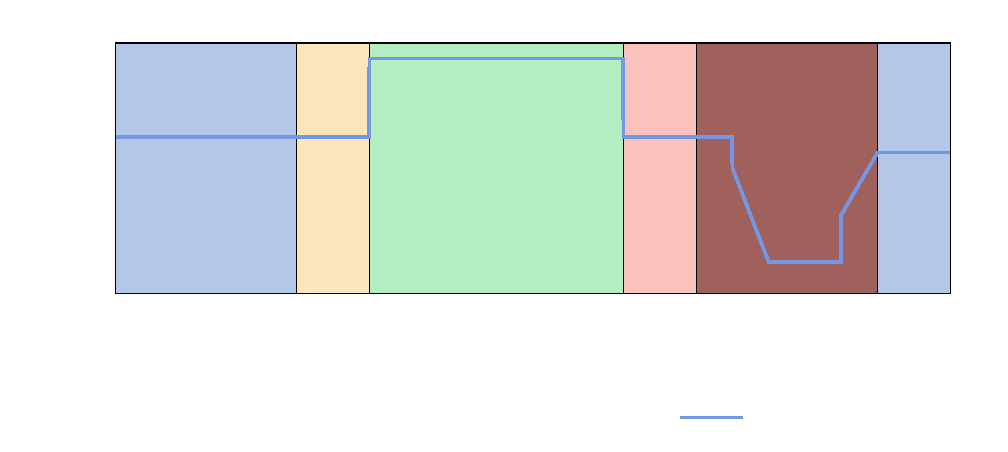
\includegraphics{Graphs/1/MiningSchedule/MiningSchedule}}%
    \gplfronttext
  \end{picture}%
\endgroup
}
	\caption[A typical operation schedule of a deep level mine.]{The typical operation schedule of a deep level mine \cite{Kriel2014Masters}.}
	\label{fig: Mining schedule}
\end{figure}
\subsection{Instrumentation and measurements}
For large industrial systems, thorough instrumentation is necessary in order to monitor performance and equipment condition throughout the system. In a mining compressed air network, instrumentation is installed to monitor flows, pressures, temperatures ,etc. Electrical instrumentation is also installed for sensing currents, power factors, voltages and power. On control valves, input/output pressures, flows and valve position are usually measured with instrumentation.	
\par
A \gls{scada} system is used to monitor and control processes throughout the mine from a control room. The \gls{scada} centralises instrumentation data from \glspl{plc} throughout the mine. The \gls{scada} can also be used to control machines and instrumentation by sending control signals to the relevant \gls{plc}.  Communication to the underground \glspl{plc} is achieved using a substantial fibre optic network.\cite{schroeder2009energy}
\clearpage
\section{Review of compressed air energy interventions in industry}
	\subsection{Preamble}
		Compressed air improvement can be obtained through intervention in either the supply or demand of compressed air \cite{Kriel2014Masters}. Improvements in supply interventions are achieved by increasing the efficiency of compressed air supply. Examples of this type of intervention include \gls{dcs}, compressor maintenance, etc. 
		\par
		Due to the size of mining compressed air networks, there is often a larger scope for improvement in air demand. Improving the demand is achieved by optimising air flow consumers, reducing leaks, etc.
		\par
	 	 This section will review compressed air supply and demand interventions that have improved energy or operation efficiency the mining industry. From the, successes and shortcomings in studies will be discussed and analysed with regard to this study.
	 	
	\subsection{Strategies to improve compressed air supply}

		\subsubsection{Compressor efficiency improvements}
		\subsubsection{Optimising compressor control}
		Compressors types and numbers can differ widely from mining compressed air systems. Compressor selection is crucial in these systems to match the correct compressors with the requirements of the system \cite{marais2010expert}.
		\par 
		In a study by Booysen \textit{et al} \cite{Booysen2012Masters} on optimising compressor control, \cite{Booysen2012Masters} found that many mines control compressors using fixed target pressure points that are much higher that required. In one system, compressors were set to a target 650 \gls{kpa} to ensure pressure underground did not fall below 500 \gls{kpa}. Using high pressure set-points can lead to excessive wasteful blow-off flow when the pressure exceeds a maximum points.
		\par
		Booysen \cite{booysen2009optimising} showed that through dynamic pressure setpoint control, matching the supply pressure with the demand, and optimal compressor selection, energy savings can be achieved. In a case study, an average power reduction of 1.07 MW was achieved. The lead to an estimated energy cost saving of R3M.
		\par 
	 	Optimising control of compressors to match the demand of the system can be complicated. \glspl{vsd} and guide vain are used to control the capacity of the system. More effective power reductions can be achieved through the use of \gls{vsd} control. Running compressors at part load reduces efficiency. From literature it shown electric motors will typical use 60-80\% of there rated power when running at $<$50\% load \cite{Saidur2010}.
		
		%\subsubsection{Air storage}
		%- booysen 1.22
		%\subsubsection{Dynamic compressor selection}
		%- van Tonder PHD
		%- van heerden 
		
		\subsubsection{Reconfiguring compressed air networks}
			A number of old mining compressed air systems  have not been adequately maintained and improved. Often they cannot sufficiently supply air to meet the demand or air is provided from non optimal sources. In a study by Bredenkamp \cite{Bredenkamp2013Masters}, reconfiguring of the air network was investigated to improve these systems.
			\par  
			In the study, Bredenkamp investigated interconnecting the compressed air systems of two mining shafts and relocating of a compressor. This strategy lead to an average power reduction of 1.7 MW and an estimated annual energy cost saving of R8.9M at the time.
			\par 
			*** \textit{Discussion of Bredenkamp} shortcomings and successes ***
			
	\subsection{Strategies to reduce compressed air demand}
	As illustrated in \cref{fig: Mining schedule}
		- Reducing leaks\\
		- Marais PhD\\
		- Snyman - investigated various Compressed air demand reduction and efficiency
		 optimisations \cite{Snyman2011Masters}.
		 
		 \subsubsection{Leakage detection}
		 
		 Air leaks are a major inefficiency in mining compressed air systems. Improving leaks is relatively easier method to  reduce air demand and improve the efficiency of the system  \cite{van2011sustaining}. Air leaks occur as a result of open pipes, fissure and breaks. Losses depend on the size of the leak and pressure in the network. \cref{fig: Leak losses} shows the theoretical airflow of through a pipe orifice as a function of leakage area and pressure\footnotemark[1]. \cite{van2011sustaining} showed that the system power consumption linearly increases with the amount of air leakage. Therefore, energy savings can be achieved through either reducing pressure or detecting and fixing leaks.
		 \begin{figure}[h]
		 	\centering
		 	\fbox{\hspace{2cm}% GNUPLOT: LaTeX picture with Postscript
\begingroup
  \makeatletter
  \providecommand\color[2][]{%
    \GenericError{(gnuplot) \space\space\space\@spaces}{%
      Package color not loaded in conjunction with
      terminal option `colourtext'%
    }{See the gnuplot documentation for explanation.%
    }{Either use 'blacktext' in gnuplot or load the package
      color.sty in LaTeX.}%
    \renewcommand\color[2][]{}%
  }%
  \providecommand\includegraphics[2][]{%
    \GenericError{(gnuplot) \space\space\space\@spaces}{%
      Package graphicx or graphics not loaded%
    }{See the gnuplot documentation for explanation.%
    }{The gnuplot epslatex terminal needs graphicx.sty or graphics.sty.}%
    \renewcommand\includegraphics[2][]{}%
  }%
  \providecommand\rotatebox[2]{#2}%
  \@ifundefined{ifGPcolor}{%
    \newif\ifGPcolor
    \GPcolortrue
  }{}%
  \@ifundefined{ifGPblacktext}{%
    \newif\ifGPblacktext
    \GPblacktextfalse
  }{}%
  % define a \g@addto@macro without @ in the name:
  \let\gplgaddtomacro\g@addto@macro
  % define empty templates for all commands taking text:
  \gdef\gplbacktext{}%
  \gdef\gplfronttext{}%
  \makeatother
  \ifGPblacktext
    % no textcolor at all
    \def\colorrgb#1{}%
    \def\colorgray#1{}%
  \else
    % gray or color?
    \ifGPcolor
      \def\colorrgb#1{\color[rgb]{#1}}%
      \def\colorgray#1{\color[gray]{#1}}%
      \expandafter\def\csname LTw\endcsname{\color{white}}%
      \expandafter\def\csname LTb\endcsname{\color{black}}%
      \expandafter\def\csname LTa\endcsname{\color{black}}%
      \expandafter\def\csname LT0\endcsname{\color[rgb]{1,0,0}}%
      \expandafter\def\csname LT1\endcsname{\color[rgb]{0,1,0}}%
      \expandafter\def\csname LT2\endcsname{\color[rgb]{0,0,1}}%
      \expandafter\def\csname LT3\endcsname{\color[rgb]{1,0,1}}%
      \expandafter\def\csname LT4\endcsname{\color[rgb]{0,1,1}}%
      \expandafter\def\csname LT5\endcsname{\color[rgb]{1,1,0}}%
      \expandafter\def\csname LT6\endcsname{\color[rgb]{0,0,0}}%
      \expandafter\def\csname LT7\endcsname{\color[rgb]{1,0.3,0}}%
      \expandafter\def\csname LT8\endcsname{\color[rgb]{0.5,0.5,0.5}}%
    \else
      % gray
      \def\colorrgb#1{\color{black}}%
      \def\colorgray#1{\color[gray]{#1}}%
      \expandafter\def\csname LTw\endcsname{\color{white}}%
      \expandafter\def\csname LTb\endcsname{\color{black}}%
      \expandafter\def\csname LTa\endcsname{\color{black}}%
      \expandafter\def\csname LT0\endcsname{\color{black}}%
      \expandafter\def\csname LT1\endcsname{\color{black}}%
      \expandafter\def\csname LT2\endcsname{\color{black}}%
      \expandafter\def\csname LT3\endcsname{\color{black}}%
      \expandafter\def\csname LT4\endcsname{\color{black}}%
      \expandafter\def\csname LT5\endcsname{\color{black}}%
      \expandafter\def\csname LT6\endcsname{\color{black}}%
      \expandafter\def\csname LT7\endcsname{\color{black}}%
      \expandafter\def\csname LT8\endcsname{\color{black}}%
    \fi
  \fi
    \setlength{\unitlength}{0.0500bp}%
    \ifx\gptboxheight\undefined%
      \newlength{\gptboxheight}%
      \newlength{\gptboxwidth}%
      \newsavebox{\gptboxtext}%
    \fi%
    \setlength{\fboxrule}{0.5pt}%
    \setlength{\fboxsep}{1pt}%
\begin{picture}(7200.00,5040.00)%
    \gplgaddtomacro\gplbacktext{%
      \colorrgb{0.00,0.00,0.00}%
      \put(1727,1050){\makebox(0,0){\strut{}$0.025$}}%
      \colorrgb{0.00,0.00,0.00}%
      \put(2545,900){\makebox(0,0){\strut{}$0.05$}}%
      \colorrgb{0.00,0.00,0.00}%
      \put(3363,750){\makebox(0,0){\strut{}$0.075$}}%
      \colorrgb{0.00,0.00,0.00}%
      \put(4180,600){\makebox(0,0){\strut{}$0.1$}}%
      \colorrgb{0.00,0.00,0.00}%
      \put(4500,755){\makebox(0,0){\strut{}$200$}}%
      \colorrgb{0.00,0.00,0.00}%
      \put(4810,927){\makebox(0,0){\strut{}$300$}}%
      \colorrgb{0.00,0.00,0.00}%
      \put(5120,1098){\makebox(0,0){\strut{}$400$}}%
      \colorrgb{0.00,0.00,0.00}%
      \put(5430,1270){\makebox(0,0){\strut{}$500$}}%
      \colorrgb{0.00,0.00,0.00}%
      \put(5750,1441){\makebox(0,0){\strut{}$600$}}%
      \colorrgb{0.00,0.00,0.00}%
      \put(6100,1613){\makebox(0,0){\strut{}$700$}}%
      \colorrgb{0.00,0.00,0.00}%
      \put(6370,1784){\makebox(0,0){\strut{}$800$}}%
      \colorrgb{0.00,0.00,0.00}%
      \put(920,2070){\makebox(0,0)[r]{\strut{}$0$}}%
      \colorrgb{0.00,0.00,0.00}%
      \put(920,2527){\makebox(0,0)[r]{\strut{}$1.5$}}%
      \colorrgb{0.00,0.00,0.00}%
      \put(920,2984){\makebox(0,0)[r]{\strut{}$3$}}%
      \colorrgb{0.00,0.00,0.00}%
      \put(920,3441){\makebox(0,0)[r]{\strut{}$4.5$}}%
    }%
    \gplgaddtomacro\gplfronttext{%
      \csname LTb\endcsname%
      \put(2198,750){\rotatebox{-9}{\makebox(0,0){\strut{}Area ($m^2$)}}}%
      \put(6029,1156){\rotatebox{30}{\makebox(0,0){\strut{}Pressure (kPa)}}}%
      \put(250,2755){\rotatebox{-270}{\makebox(0,0){\strut{}Flow (kg/s)}}}%
    }%
    \gplbacktext
    \put(0,0){\fbox{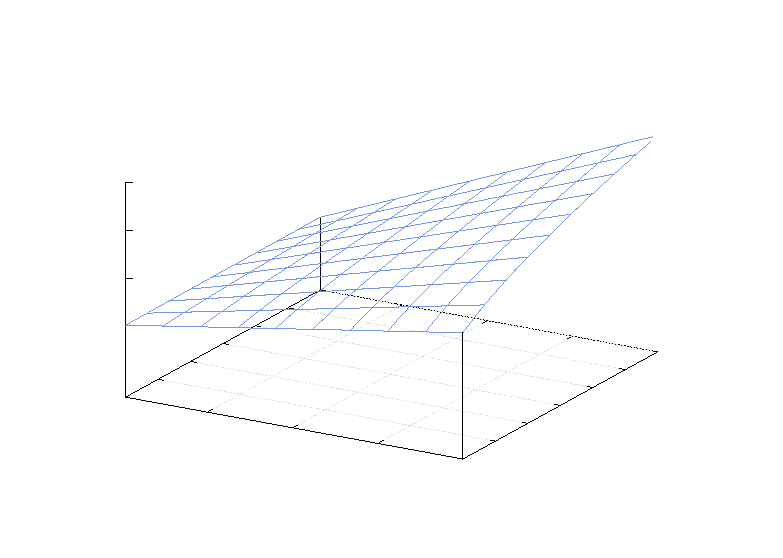
\includegraphics[trim=0 0 0.1cm 0, clip]{Graphs/2/Leak2/Leak2}}}%
    \gplfronttext
  \end{picture}%
\endgroup
\hspace{2cm}}
		 	\caption[The leakage flow as a function of inlet pressure and leakage area]{ The leakage flow as a function of inlet pressure and leakage area\protect\footnotemark[1].}
		 	\label{fig: Leak losses}
		 \end{figure}
	 \footnotetext[1]{efunda, "Orifice Flowmeter Calculator." [Online] \url{http://www.efunda.com/formulae/fluids/calc_orifice_flowmeter.cfm}, [Accessed 18 October 2016].}
	 \par 
		 Leaks are often not easily detected through visual methods. In industry, a number of techniques are employed to detect air leaks. Pascoe \cite{Pascoe2016Masters} and van Tonder \cite{vanTonder2010Masters} summarised these strategies as follows:
		 \begin{itemize}
		 	\item Audible detection (Walk and report)
		 	\item Ultrasonic detection
		 	\item Detection through intelligent systems
		 	\item Pigging
		 	\item Soap water and dyes
		 \end{itemize}
	 	 These methods are time and resource intensive and many mines do not actively employ dedicated leakage detection and repair teams. Marais \textit{et al} \cite{marais2009increased} investigated streamlining the leakage detection and repair process to increase energy savings through the use of \gls{calds}. The system was developed to allow centralised mobile leakage reporting. Usage of \gls{calds} in mines resulted in an increased leak detection rate. One mine reporting 24 leaks in a single month. It was noted in the study that there difficulty quantifying the actual energy savings of the leakage repairs due to other intervention occurring simultaneously.	
		 
		 \subsubsection{Underground control valves optimisation}
		 Many mines utilise automated valves at critical locations or levels in the compressed air network. These valves control the pressure, restricting airflow from that point in the air network. Restricting airflow reduces losses resultant from network inefficiencies and leaks.
		 \par 
		 Kleingeld and Marais \cite{kleingeld2010high} found that optimising control valve control on mining levels can conservatively lead to between 20\% on mines where no control valves are installed. For systems that already have some form of network control, between 10 and 15\% savings can conservatively be achieved.
		 \par 
		 From literature, the advantage of control valve optimisation is the significant savings that can be achieved with relatively short set-up up time. Savings can be achieved incrementally with each control valve installation. Studies did not look at accurate estimations of savings or the shaft pressure improvements that result from control valve optimisation.	 
		\subsubsection{Improving pneumatic rock drill efficiency}
		 Pneumatic rock drills are on of the largest air consumers in a mine. However Pneumatic drilling systems are convert energy very inefficiently. Replacing pneumatic drills with more efficient alternatives such as hydraulic or pneumatic drills would lead to large energy savings \cite{Pascoe2016Masters}**.  Alternatively improving the efficiency or pneumatic drilling can have a significant energy impact on the system, without the cost and safety concerns of alternative drilling technologies.
		 \par 
		  In a study by  Bester \textit{et al.} \cite{bester2013effect} looking at the effect of compressed air pressure on energy demand. Bester showed that between 2002 and 2013 compressed air and energy consumption per tonne of ore produced had steadily increased. This is illustrated  in \cref{fig: Compressed energy and air flow per ton}. 
		 The increase of air consumption per \gls{t} was a result of reduced air pressure at the mining areas. This causes the drilling rate to drop leading to higher air consumption. Pressure measurements as low as 300 \gls{kpa} were recorded in these areas. Before 2002 the drilling pressure at the mining section (stopes), was maintained above 500 \gls{kpa} at most mines. 
		 \par 
		 \begin{figure}[h]
		 	\centering
		 	% GNUPLOT: LaTeX picture with Postscript
\begingroup
  \makeatletter
  \providecommand\color[2][]{%
    \GenericError{(gnuplot) \space\space\space\@spaces}{%
      Package color not loaded in conjunction with
      terminal option `colourtext'%
    }{See the gnuplot documentation for explanation.%
    }{Either use 'blacktext' in gnuplot or load the package
      color.sty in LaTeX.}%
    \renewcommand\color[2][]{}%
  }%
  \providecommand\includegraphics[2][]{%
    \GenericError{(gnuplot) \space\space\space\@spaces}{%
      Package graphicx or graphics not loaded%
    }{See the gnuplot documentation for explanation.%
    }{The gnuplot epslatex terminal needs graphicx.sty or graphics.sty.}%
    \renewcommand\includegraphics[2][]{}%
  }%
  \providecommand\rotatebox[2]{#2}%
  \@ifundefined{ifGPcolor}{%
    \newif\ifGPcolor
    \GPcolortrue
  }{}%
  \@ifundefined{ifGPblacktext}{%
    \newif\ifGPblacktext
    \GPblacktextfalse
  }{}%
  % define a \g@addto@macro without @ in the name:
  \let\gplgaddtomacro\g@addto@macro
  % define empty templates for all commands taking text:
  \gdef\gplbacktext{}%
  \gdef\gplfronttext{}%
  \makeatother
  \ifGPblacktext
    % no textcolor at all
    \def\colorrgb#1{}%
    \def\colorgray#1{}%
  \else
    % gray or color?
    \ifGPcolor
      \def\colorrgb#1{\color[rgb]{#1}}%
      \def\colorgray#1{\color[gray]{#1}}%
      \expandafter\def\csname LTw\endcsname{\color{white}}%
      \expandafter\def\csname LTb\endcsname{\color{black}}%
      \expandafter\def\csname LTa\endcsname{\color{black}}%
      \expandafter\def\csname LT0\endcsname{\color[rgb]{1,0,0}}%
      \expandafter\def\csname LT1\endcsname{\color[rgb]{0,1,0}}%
      \expandafter\def\csname LT2\endcsname{\color[rgb]{0,0,1}}%
      \expandafter\def\csname LT3\endcsname{\color[rgb]{1,0,1}}%
      \expandafter\def\csname LT4\endcsname{\color[rgb]{0,1,1}}%
      \expandafter\def\csname LT5\endcsname{\color[rgb]{1,1,0}}%
      \expandafter\def\csname LT6\endcsname{\color[rgb]{0,0,0}}%
      \expandafter\def\csname LT7\endcsname{\color[rgb]{1,0.3,0}}%
      \expandafter\def\csname LT8\endcsname{\color[rgb]{0.5,0.5,0.5}}%
    \else
      % gray
      \def\colorrgb#1{\color{black}}%
      \def\colorgray#1{\color[gray]{#1}}%
      \expandafter\def\csname LTw\endcsname{\color{white}}%
      \expandafter\def\csname LTb\endcsname{\color{black}}%
      \expandafter\def\csname LTa\endcsname{\color{black}}%
      \expandafter\def\csname LT0\endcsname{\color{black}}%
      \expandafter\def\csname LT1\endcsname{\color{black}}%
      \expandafter\def\csname LT2\endcsname{\color{black}}%
      \expandafter\def\csname LT3\endcsname{\color{black}}%
      \expandafter\def\csname LT4\endcsname{\color{black}}%
      \expandafter\def\csname LT5\endcsname{\color{black}}%
      \expandafter\def\csname LT6\endcsname{\color{black}}%
      \expandafter\def\csname LT7\endcsname{\color{black}}%
      \expandafter\def\csname LT8\endcsname{\color{black}}%
    \fi
  \fi
    \setlength{\unitlength}{0.0500bp}%
    \ifx\gptboxheight\undefined%
      \newlength{\gptboxheight}%
      \newlength{\gptboxwidth}%
      \newsavebox{\gptboxtext}%
    \fi%
    \setlength{\fboxrule}{0.5pt}%
    \setlength{\fboxsep}{1pt}%
\begin{picture}(9360.00,4032.00)%
    \gplgaddtomacro\gplbacktext{%
      \colorrgb{0.42,0.42,0.42}%
      \put(682,924){\makebox(0,0)[r]{\strut{}$0$}}%
      \colorrgb{0.42,0.42,0.42}%
      \put(682,1230){\makebox(0,0)[r]{\strut{}$5$}}%
      \colorrgb{0.42,0.42,0.42}%
      \put(682,1536){\makebox(0,0)[r]{\strut{}$10$}}%
      \colorrgb{0.42,0.42,0.42}%
      \put(682,1842){\makebox(0,0)[r]{\strut{}$15$}}%
      \colorrgb{0.42,0.42,0.42}%
      \put(682,2148){\makebox(0,0)[r]{\strut{}$20$}}%
      \colorrgb{0.42,0.42,0.42}%
      \put(682,2453){\makebox(0,0)[r]{\strut{}$25$}}%
      \colorrgb{0.42,0.42,0.42}%
      \put(682,2759){\makebox(0,0)[r]{\strut{}$30$}}%
      \colorrgb{0.42,0.42,0.42}%
      \put(682,3065){\makebox(0,0)[r]{\strut{}$35$}}%
      \colorrgb{0.42,0.42,0.42}%
      \put(682,3371){\makebox(0,0)[r]{\strut{}$40$}}%
      \colorrgb{0.42,0.42,0.42}%
      \put(814,704){\makebox(0,0){\strut{}$2002$}}%
      \colorrgb{0.42,0.42,0.42}%
      \put(2025,704){\makebox(0,0){\strut{}$2004$}}%
      \colorrgb{0.42,0.42,0.42}%
      \put(3237,704){\makebox(0,0){\strut{}$2006$}}%
      \colorrgb{0.42,0.42,0.42}%
      \put(4448,704){\makebox(0,0){\strut{}$2008$}}%
      \colorrgb{0.42,0.42,0.42}%
      \put(5659,704){\makebox(0,0){\strut{}$2010$}}%
      \colorrgb{0.42,0.42,0.42}%
      \put(6871,704){\makebox(0,0){\strut{}$2012$}}%
      \colorrgb{0.42,0.42,0.42}%
      \put(8082,704){\makebox(0,0){\strut{}$2014$}}%
      \colorrgb{0.42,0.42,0.42}%
      \put(8214,924){\makebox(0,0)[l]{\strut{}$0$}}%
      \colorrgb{0.42,0.42,0.42}%
      \put(8214,1230){\makebox(0,0)[l]{\strut{}$50$}}%
      \colorrgb{0.42,0.42,0.42}%
      \put(8214,1536){\makebox(0,0)[l]{\strut{}$100$}}%
      \colorrgb{0.42,0.42,0.42}%
      \put(8214,1842){\makebox(0,0)[l]{\strut{}$150$}}%
      \colorrgb{0.42,0.42,0.42}%
      \put(8214,2148){\makebox(0,0)[l]{\strut{}$200$}}%
      \colorrgb{0.42,0.42,0.42}%
      \put(8214,2453){\makebox(0,0)[l]{\strut{}$250$}}%
      \colorrgb{0.42,0.42,0.42}%
      \put(8214,2759){\makebox(0,0)[l]{\strut{}$300$}}%
      \colorrgb{0.42,0.42,0.42}%
      \put(8214,3065){\makebox(0,0)[l]{\strut{}$350$}}%
      \colorrgb{0.42,0.42,0.42}%
      \put(8214,3371){\makebox(0,0)[l]{\strut{}$400$}}%
    }%
    \gplgaddtomacro\gplfronttext{%
      \csname LTb\endcsname%
      \put(176,2147){\rotatebox{-270}{\makebox(0,0){\strut{}kWh/t}}}%
      \put(8851,2147){\rotatebox{-270}{\makebox(0,0){\strut{}$m^3$/t}}}%
      \put(4448,374){\makebox(0,0){\strut{}Year}}%
      \put(4448,3701){\makebox(0,0){\strut{}Compressed air energy and Volume consumed per ton}}%
      \csname LTb\endcsname%
      \put(3593,173){\makebox(0,0)[r]{\strut{}Energy per Ton (kWh/t)}}%
      \csname LTb\endcsname%
      \put(7352,173){\makebox(0,0)[r]{\strut{}Volume per Ton ($m^3$/t)}}%
    }%
    \gplbacktext
    \put(0,0){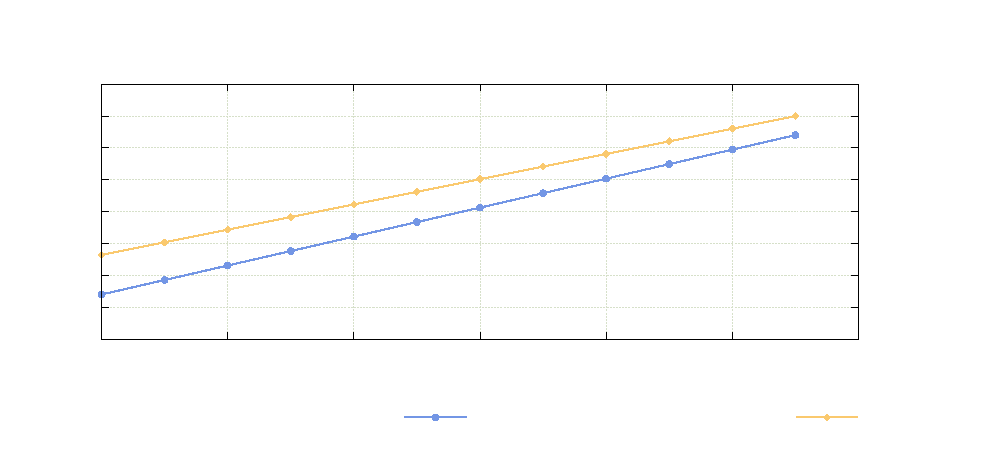
\includegraphics{Graphs/1/EVperT/EVperT}}%
    \gplfronttext
  \end{picture}%
\endgroup

		 	\caption[The Compressed air energy and flow consumed per T of ore produced.]{The Compressed air energy and flow consumed per T of ore produced. Adopted from Bester \textit{et al.} \cite{bester2013effect}.}
		 	\label{fig: Compressed energy and air flow per ton}
		 \end{figure}
		 From literature, it is shown that lowering the pressure reduces the efficiency and drill rate of rock drilling, leading to higher air consumption. Interventions that reduce systemic air losses or optimise supply can increase the pressure operating pressure. Increased pressure, during the drilling shift, may add more value than the energy cost savings that can be achieved at a lower pressure.
	\subsection{Summary}
\clearpage

\section{Use of simulations to identify improvements in mining systems}
	\subsection{Preamble}
	The value of simulation in  the mining industry has been shown through its use in \gls{dsm} initiatives. Simulation has been used to identify savings strategies for water reticulation cooling, compressed air and ventilation. This section will summarise the the work that has been done in industry. From this the successes and shortcomings of previous work will be discussed.
	
		\subsection{Estimating techniques used for energy savings on mining systems }
		Estimation of energy savings has been used in literature to obtain the potential energy impact that can be achieved for a system. Before new tools allowed for quick development of simplified simulation models, estimation techniques were frequently used to determine the feasibility of energy interventions on mining systems. The problem with an estimation approach is that they typically rely on simplified models with high resultant error.
		\par 
		- Snyman estimated improvements using historical data.\cite{Snyman2011Masters}\\
		 
		
		\subsubsection{Benchmark modelling}
		YEha  \cite{Cilliers2015PHD} developed \enquote{best practice models} using the \gls{cols} benchmarking method. These models provide an energy benchmark that can be used to identify the scope for energy improvements on a system. An example of a benchmark model for a mining compressed air system is shown in \cref{eq: COLS}. The model shows that energy required is dependent on the quantity of ore mined and the depth of the mine. \cite{Cilliers2015PHD} also developed benchmark models for mine cooling, water reticulation and ventilation systems.

		\begin{figure}[h!]
			\centering
			\fbox{\hspace{2cm}% GNUPLOT: LaTeX picture with Postscript
\begingroup
  \makeatletter
  \providecommand\color[2][]{%
    \GenericError{(gnuplot) \space\space\space\@spaces}{%
      Package color not loaded in conjunction with
      terminal option `colourtext'%
    }{See the gnuplot documentation for explanation.%
    }{Either use 'blacktext' in gnuplot or load the package
      color.sty in LaTeX.}%
    \renewcommand\color[2][]{}%
  }%
  \providecommand\includegraphics[2][]{%
    \GenericError{(gnuplot) \space\space\space\@spaces}{%
      Package graphicx or graphics not loaded%
    }{See the gnuplot documentation for explanation.%
    }{The gnuplot epslatex terminal needs graphicx.sty or graphics.sty.}%
    \renewcommand\includegraphics[2][]{}%
  }%
  \providecommand\rotatebox[2]{#2}%
  \@ifundefined{ifGPcolor}{%
    \newif\ifGPcolor
    \GPcolortrue
  }{}%
  \@ifundefined{ifGPblacktext}{%
    \newif\ifGPblacktext
    \GPblacktextfalse
  }{}%
  % define a \g@addto@macro without @ in the name:
  \let\gplgaddtomacro\g@addto@macro
  % define empty templates for all commands taking text:
  \gdef\gplbacktext{}%
  \gdef\gplfronttext{}%
  \makeatother
  \ifGPblacktext
    % no textcolor at all
    \def\colorrgb#1{}%
    \def\colorgray#1{}%
  \else
    % gray or color?
    \ifGPcolor
      \def\colorrgb#1{\color[rgb]{#1}}%
      \def\colorgray#1{\color[gray]{#1}}%
      \expandafter\def\csname LTw\endcsname{\color{white}}%
      \expandafter\def\csname LTb\endcsname{\color{black}}%
      \expandafter\def\csname LTa\endcsname{\color{black}}%
      \expandafter\def\csname LT0\endcsname{\color[rgb]{1,0,0}}%
      \expandafter\def\csname LT1\endcsname{\color[rgb]{0,1,0}}%
      \expandafter\def\csname LT2\endcsname{\color[rgb]{0,0,1}}%
      \expandafter\def\csname LT3\endcsname{\color[rgb]{1,0,1}}%
      \expandafter\def\csname LT4\endcsname{\color[rgb]{0,1,1}}%
      \expandafter\def\csname LT5\endcsname{\color[rgb]{1,1,0}}%
      \expandafter\def\csname LT6\endcsname{\color[rgb]{0,0,0}}%
      \expandafter\def\csname LT7\endcsname{\color[rgb]{1,0.3,0}}%
      \expandafter\def\csname LT8\endcsname{\color[rgb]{0.5,0.5,0.5}}%
    \else
      % gray
      \def\colorrgb#1{\color{black}}%
      \def\colorgray#1{\color[gray]{#1}}%
      \expandafter\def\csname LTw\endcsname{\color{white}}%
      \expandafter\def\csname LTb\endcsname{\color{black}}%
      \expandafter\def\csname LTa\endcsname{\color{black}}%
      \expandafter\def\csname LT0\endcsname{\color{black}}%
      \expandafter\def\csname LT1\endcsname{\color{black}}%
      \expandafter\def\csname LT2\endcsname{\color{black}}%
      \expandafter\def\csname LT3\endcsname{\color{black}}%
      \expandafter\def\csname LT4\endcsname{\color{black}}%
      \expandafter\def\csname LT5\endcsname{\color{black}}%
      \expandafter\def\csname LT6\endcsname{\color{black}}%
      \expandafter\def\csname LT7\endcsname{\color{black}}%
      \expandafter\def\csname LT8\endcsname{\color{black}}%
    \fi
  \fi
    \setlength{\unitlength}{0.0500bp}%
    \ifx\gptboxheight\undefined%
      \newlength{\gptboxheight}%
      \newlength{\gptboxwidth}%
      \newsavebox{\gptboxtext}%
    \fi%
    \setlength{\fboxrule}{0.5pt}%
    \setlength{\fboxsep}{1pt}%
\begin{picture}(7000.00,5200.00)%
    \gplgaddtomacro\gplbacktext{%
      \colorrgb{0.00,0.00,0.00}%
      \put(936,1465){\makebox(0,0){\strut{}$0$}}%
      \colorrgb{0.00,0.00,0.00}%
      \put(1745,1325){\makebox(0,0){\strut{}$1$}}%
      \colorrgb{0.00,0.00,0.00}%
      \put(2555,1184){\makebox(0,0){\strut{}$2$}}%
      \colorrgb{0.00,0.00,0.00}%
      \put(3365,1043){\makebox(0,0){\strut{}$3$}}%
      \colorrgb{0.00,0.00,0.00}%
      \put(4174,903){\makebox(0,0){\strut{}$4$}}%
      \colorrgb{0.00,0.00,0.00}%
      \put(4600,965){\makebox(0,0){\strut{}$0$}}%
      \colorrgb{0.00,0.00,0.00}%
      \put(4850,1087){\makebox(0,0){\strut{}$20$}}%
      \colorrgb{0.00,0.00,0.00}%
      \put(5050,1208){\makebox(0,0){\strut{}$40$}}%
      \colorrgb{0.00,0.00,0.00}%
      \put(5300,1330){\makebox(0,0){\strut{}$60$}}%
      \colorrgb{0.00,0.00,0.00}%
      \put(5530,1452){\makebox(0,0){\strut{}$80$}}%
      \colorrgb{0.00,0.00,0.00}%
      \put(5770,1574){\makebox(0,0){\strut{}$100$}}%
      \colorrgb{0.00,0.00,0.00}%
      \put(6000,1695){\makebox(0,0){\strut{}$120$}}%
      \colorrgb{0.00,0.00,0.00}%
      \put(6230,1817){\makebox(0,0){\strut{}$140$}}%
      \colorrgb{0.00,0.00,0.00}%
      \put(6470,1939){\makebox(0,0){\strut{}$160$}}%
      \colorrgb{0.00,0.00,0.00}%
      \put(920,2210){\makebox(0,0)[r]{\strut{}$0$}}%
      \colorrgb{0.00,0.00,0.00}%
      \put(920,2470){\makebox(0,0)[r]{\strut{}$2$}}%
      \colorrgb{0.00,0.00,0.00}%
      \put(920,2729){\makebox(0,0)[r]{\strut{}$4$}}%
      \colorrgb{0.00,0.00,0.00}%
      \put(920,2988){\makebox(0,0)[r]{\strut{}$6$}}%
      \colorrgb{0.00,0.00,0.00}%
      \put(920,3248){\makebox(0,0)[r]{\strut{}$8$}}%
      \colorrgb{0.00,0.00,0.00}%
      \put(920,3508){\makebox(0,0)[r]{\strut{}$10$}}%
    }%
    \gplgaddtomacro\gplfronttext{%
    	\csname LTb\endcsname%
    	\put(5456,200){\makebox(0,0)[r]{\strut{}$E_{comp} = 1.51\cdot Z + 33.36\cdot T - 1930.21$}}%  	
    	\csname LTb\endcsname%
    	\put(6000,1400){\rotatebox{28}{\makebox(0,0){\strut{} T - Mined ore ($kT$)}}}%
    	\put(2100,1000){\rotatebox{-9}{\makebox(0,0){\strut{}Z - Mine depth ($km$)}}}%
    	\put(600,2858){\rotatebox{-270}{\makebox(0,0){\strut{}Benchmark energy (GWhr)}}}%
    }%
    \gplbacktext
    \put(0,0){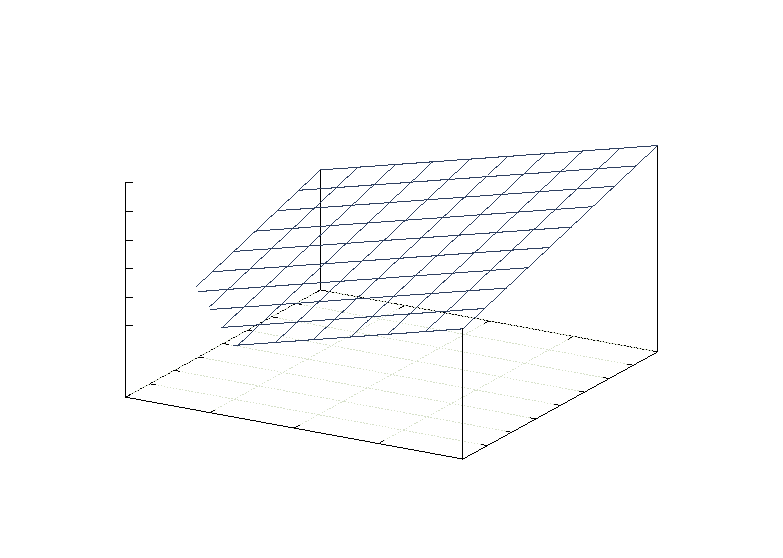
\includegraphics[trim=0 -0.51cm 0 0 ]{Graphs/2/Benchmark/Benchmark}}%
    \gplfronttext
  \end{picture}%
\endgroup
\hspace{2cm}}
			\caption{ }
			\label{fig: 3D Benchmark}
		\end{figure}
	%%%%%%%%%%%%%%%%%%%%%%%%%% Equation %%%%%%%%%%%%%%%%%%%%%%%%%%%%%
	%	\begin{equation}
	%	\label{eq: COLS}
	%	E_{comp} = 1.51\cdot Z + 33.36\cdot T - 1930.21
	%	\end{equation}			
	%%%%%%%%%%%%%%%%%%%%%%%%%%%%%%%%%%%%%%%%%%%%%%%%%%%%%%%%%%%%%%%%%%
	\subsection{Value of simulation in mining DSM}
	Van Niekerk \cite{van2013value},\cite{vanNiekerk2012Value} investigated the value of simulation models in mine \gls{dsm} projects. Van Niekerk developed simulation models for compressed air and water reticulation systems using KYPipes's gas simulation engine. \\
	
	\subsubsection{Mine cooling systems}
	Simulation has been used in studies as a tool to improve mine cooling. Holman \cite{Holman2014Masters} investigated improvements to mine cooling systems that improve performance and efficiency. In the study \cite{Holman2014Masters}  used simplified \gls{ptb}  simulation models to investigate cooling interventions.
	\par 
	The scenario Holman simulated showed potential  average power reduction of 136 kW  which would lead to an annual energy cost saving of R0.55M. The study could be improved by increasing accuracy of the simulation. Power difference of as high as 31\% between the simulation and actual were observed for some time periods.
	\subsubsection{Mine de-watering systems}
	
	\subsubsection{Mine compressed air systems}
		
	\subsection{Simulation procedures}
		- Philip
		- Kriel masters\\
		\subsubsection{Periodic simulation}
 	\subsection{Simulation model verification strategies}
 	From literature, methods of verifying simulation were analysed. Most studies utilised a comparison calculation strategy to calculate a model accuracy or error. %Two calculation methods identified were \emph{Average difference method} and \emph{average percentage difference}. 
 		\subsubsection{Mean residual difference method}
 			The average difference method looks at the average for the data points in the actual and simulated time series.  The error \% is then calculated with \cref{eq: Average difference}. The error is then calculated as a percentage by dividing the error by the Actual values, \cref{eq: Average difference}.
 			
 			\begin{equation}
 			\label{eq: AMean absolute}
 			\tilde{R} = \left| \dfrac{1}{N} \sum_{n=1}^{N}{ \left( A_{n} - S_{n}\right)}  \right|
 			\end{equation}
 To get	an error percentage, the equation is rewritten:	
 			\begin{equation}
 				\label{eq: Average difference}
 				Err_{\%} = \left| \dfrac{1}{N} \sum_{n=1}^{N}{ \left(\dfrac{ A_{n} - S_{n}}{A_n}\right)}  \right|
 			\end{equation}
 			Where: \par 
 				\begin{table}[h!]
 					\centering
 					\begin{tabular}{cl}
 						$A$ & Actual system time series \\
 						$S$ & Simulation time series \\
 						$n$ & sample \\
 						$N$ & Number of samples in simulation period \\
 					\end{tabular} 
 				\end{table}	
 			A major disadvantage of this method is the the errors for individual points are cancelled out. The result therefore can not lead to conclusive deductions.\cite{sarin2010comparing} This strategy is not recommended if used alone to verify data.
 			
 			
 		\subsubsection{Mean absolute error method}
 		The relative error method follows a similar calculation as in the Average difference method. However, as shown in \cref{eq: Relative error}, the error is calculated individually for each point in the series. The average of the individually errors is the resultant error, \cref{eq: Relative error 2}. To obtain the error percentage, each error is divided by the Actual value at that time step as in \cref{eq: Relative error}.
 		\begin{equation}
 		\label{eq: Relative error 2}
 		MAE = \dfrac{1}{N}\sum_{n=1}^{N}{\left|A_{n} - S_{n}\right| }
 		\end{equation}
 			To get	an error percentage, the equation is rewritten:	
 			\begin{equation}
 			\label{eq: Relative error}
 			Err_{\%} = \dfrac{1}{N}\sum_{n=1}^{N}{\left|\dfrac{A_{n} - S_{n}}{A_{n}}\right| }
 			\end{equation}
 			Where: \par
 			\begin{table}[h!]
 				\centering
 				\begin{tabular}{cl}
 					$A$ & Actual system time series  \\
 					$M$ & Simulation  time series  \\
 					$n$ & sample \\
 					$N$ & Number of samples in simulation period \\
 				\end{tabular} 
 			\end{table}	
 		Yu-jie Xu \cite{xu2016modeling}
 		\par 
 		\subsubsection{Comparing verification methods}
 		The difference between the verification strategies is best shown using an example. Figure \cref{fig:Philipp Difference verify} Shows a comparison between a simulation model's output power and the actual power of the system over a 24 hour period. In a study by \cite{Mare2016PhD}, the average \% difference method, \cref{eq: Average difference}, was used to calculate the accuracy of a simulation model. The average of the two power profiles were similar, leading to a calculated error of 1.17\%. However, the Relative error method, \cref{eq: Relative error}, applied to the same data the results in a error of 15.2\%. 
 		
 	\begin{figure}[h!]
 		\centering
 		% GNUPLOT: LaTeX picture with Postscript
\begingroup
  \makeatletter
  \providecommand\color[2][]{%
    \GenericError{(gnuplot) \space\space\space\@spaces}{%
      Package color not loaded in conjunction with
      terminal option `colourtext'%
    }{See the gnuplot documentation for explanation.%
    }{Either use 'blacktext' in gnuplot or load the package
      color.sty in LaTeX.}%
    \renewcommand\color[2][]{}%
  }%
  \providecommand\includegraphics[2][]{%
    \GenericError{(gnuplot) \space\space\space\@spaces}{%
      Package graphicx or graphics not loaded%
    }{See the gnuplot documentation for explanation.%
    }{The gnuplot epslatex terminal needs graphicx.sty or graphics.sty.}%
    \renewcommand\includegraphics[2][]{}%
  }%
  \providecommand\rotatebox[2]{#2}%
  \@ifundefined{ifGPcolor}{%
    \newif\ifGPcolor
    \GPcolortrue
  }{}%
  \@ifundefined{ifGPblacktext}{%
    \newif\ifGPblacktext
    \GPblacktextfalse
  }{}%
  % define a \g@addto@macro without @ in the name:
  \let\gplgaddtomacro\g@addto@macro
  % define empty templates for all commands taking text:
  \gdef\gplbacktext{}%
  \gdef\gplfronttext{}%
  \makeatother
  \ifGPblacktext
    % no textcolor at all
    \def\colorrgb#1{}%
    \def\colorgray#1{}%
  \else
    % gray or color?
    \ifGPcolor
      \def\colorrgb#1{\color[rgb]{#1}}%
      \def\colorgray#1{\color[gray]{#1}}%
      \expandafter\def\csname LTw\endcsname{\color{white}}%
      \expandafter\def\csname LTb\endcsname{\color{black}}%
      \expandafter\def\csname LTa\endcsname{\color{black}}%
      \expandafter\def\csname LT0\endcsname{\color[rgb]{1,0,0}}%
      \expandafter\def\csname LT1\endcsname{\color[rgb]{0,1,0}}%
      \expandafter\def\csname LT2\endcsname{\color[rgb]{0,0,1}}%
      \expandafter\def\csname LT3\endcsname{\color[rgb]{1,0,1}}%
      \expandafter\def\csname LT4\endcsname{\color[rgb]{0,1,1}}%
      \expandafter\def\csname LT5\endcsname{\color[rgb]{1,1,0}}%
      \expandafter\def\csname LT6\endcsname{\color[rgb]{0,0,0}}%
      \expandafter\def\csname LT7\endcsname{\color[rgb]{1,0.3,0}}%
      \expandafter\def\csname LT8\endcsname{\color[rgb]{0.5,0.5,0.5}}%
    \else
      % gray
      \def\colorrgb#1{\color{black}}%
      \def\colorgray#1{\color[gray]{#1}}%
      \expandafter\def\csname LTw\endcsname{\color{white}}%
      \expandafter\def\csname LTb\endcsname{\color{black}}%
      \expandafter\def\csname LTa\endcsname{\color{black}}%
      \expandafter\def\csname LT0\endcsname{\color{black}}%
      \expandafter\def\csname LT1\endcsname{\color{black}}%
      \expandafter\def\csname LT2\endcsname{\color{black}}%
      \expandafter\def\csname LT3\endcsname{\color{black}}%
      \expandafter\def\csname LT4\endcsname{\color{black}}%
      \expandafter\def\csname LT5\endcsname{\color{black}}%
      \expandafter\def\csname LT6\endcsname{\color{black}}%
      \expandafter\def\csname LT7\endcsname{\color{black}}%
      \expandafter\def\csname LT8\endcsname{\color{black}}%
    \fi
  \fi
    \setlength{\unitlength}{0.0500bp}%
    \ifx\gptboxheight\undefined%
      \newlength{\gptboxheight}%
      \newlength{\gptboxwidth}%
      \newsavebox{\gptboxtext}%
    \fi%
    \setlength{\fboxrule}{0.5pt}%
    \setlength{\fboxsep}{1pt}%
\begin{picture}(9360.00,4536.00)%
    \gplgaddtomacro\gplbacktext{%
      \colorrgb{0.00,0.00,0.00}%
      \put(682,1584){\makebox(0,0)[r]{\strut{}$0$}}%
      \colorrgb{0.00,0.00,0.00}%
      \put(682,1853){\makebox(0,0)[r]{\strut{}$1$}}%
      \colorrgb{0.00,0.00,0.00}%
      \put(682,2121){\makebox(0,0)[r]{\strut{}$2$}}%
      \colorrgb{0.00,0.00,0.00}%
      \put(682,2390){\makebox(0,0)[r]{\strut{}$3$}}%
      \colorrgb{0.00,0.00,0.00}%
      \put(682,2659){\makebox(0,0)[r]{\strut{}$4$}}%
      \colorrgb{0.00,0.00,0.00}%
      \put(682,2927){\makebox(0,0)[r]{\strut{}$5$}}%
      \colorrgb{0.00,0.00,0.00}%
      \put(682,3196){\makebox(0,0)[r]{\strut{}$6$}}%
      \colorrgb{0.00,0.00,0.00}%
      \put(682,3465){\makebox(0,0)[r]{\strut{}$7$}}%
      \colorrgb{0.00,0.00,0.00}%
      \put(682,3734){\makebox(0,0)[r]{\strut{}$8$}}%
      \colorrgb{0.00,0.00,0.00}%
      \put(682,4002){\makebox(0,0)[r]{\strut{}$9$}}%
      \colorrgb{0.00,0.00,0.00}%
      \put(682,4271){\makebox(0,0)[r]{\strut{}$10$}}%
      \colorrgb{0.00,0.00,0.00}%
      \put(1286,1364){\makebox(0,0){\strut{}02:00}}%
      \colorrgb{0.00,0.00,0.00}%
      \put(1916,1364){\makebox(0,0){\strut{}04:00}}%
      \colorrgb{0.00,0.00,0.00}%
      \put(2546,1364){\makebox(0,0){\strut{}06:00}}%
      \colorrgb{0.00,0.00,0.00}%
      \put(3176,1364){\makebox(0,0){\strut{}08:00}}%
      \colorrgb{0.00,0.00,0.00}%
      \put(3805,1364){\makebox(0,0){\strut{}10:00}}%
      \colorrgb{0.00,0.00,0.00}%
      \put(4435,1364){\makebox(0,0){\strut{}12:00}}%
      \colorrgb{0.00,0.00,0.00}%
      \put(5065,1364){\makebox(0,0){\strut{}14:00}}%
      \colorrgb{0.00,0.00,0.00}%
      \put(5695,1364){\makebox(0,0){\strut{}16:00}}%
      \colorrgb{0.00,0.00,0.00}%
      \put(6325,1364){\makebox(0,0){\strut{}18:00}}%
      \colorrgb{0.00,0.00,0.00}%
      \put(6954,1364){\makebox(0,0){\strut{}20:00}}%
      \colorrgb{0.00,0.00,0.00}%
      \put(7584,1364){\makebox(0,0){\strut{}22:00}}%
      \colorrgb{0.00,0.00,0.00}%
      \put(8214,1364){\makebox(0,0){\strut{}00:00}}%
      \colorrgb{0.00,0.00,0.00}%
      \put(8346,1584){\makebox(0,0)[l]{\strut{}$0$}}%
      \colorrgb{0.00,0.00,0.00}%
      \put(8346,1853){\makebox(0,0)[l]{\strut{}$1$}}%
      \colorrgb{0.00,0.00,0.00}%
      \put(8346,2121){\makebox(0,0)[l]{\strut{}$2$}}%
      \colorrgb{0.00,0.00,0.00}%
      \put(8346,2390){\makebox(0,0)[l]{\strut{}$3$}}%
      \colorrgb{0.00,0.00,0.00}%
      \put(8346,2659){\makebox(0,0)[l]{\strut{}$4$}}%
      \colorrgb{0.00,0.00,0.00}%
      \put(8346,2927){\makebox(0,0)[l]{\strut{}$5$}}%
      \colorrgb{0.00,0.00,0.00}%
      \put(8346,3196){\makebox(0,0)[l]{\strut{}$6$}}%
      \colorrgb{0.00,0.00,0.00}%
      \put(8346,3465){\makebox(0,0)[l]{\strut{}$7$}}%
      \colorrgb{0.00,0.00,0.00}%
      \put(8346,3734){\makebox(0,0)[l]{\strut{}$8$}}%
      \colorrgb{0.00,0.00,0.00}%
      \put(8346,4002){\makebox(0,0)[l]{\strut{}$9$}}%
      \colorrgb{0.00,0.00,0.00}%
      \put(8346,4271){\makebox(0,0)[l]{\strut{}$10$}}%
      \csname LTb\endcsname%
      \put(1024,3000){\makebox(0,0)[l]{\strut{}\shortstack{Residual \\ difference}}}%
      \put(1024,1745){\makebox(0,0)[l]{\strut{}MAE}}%
      \put(1024,2014){\makebox(0,0)[l]{\strut{}MSE}}%
    }%
    \gplgaddtomacro\gplfronttext{%
      \csname LTb\endcsname%
      \put(176,2927){\rotatebox{-270}{\makebox(0,0){\strut{}Power $(MW)$}}}%
      \put(8851,2600){\rotatebox{-270}{\makebox(0,0){\strut{} Relative $Err_{\%} $}}}%
      \put(4514,1034){\makebox(0,0){\strut{}Time of use}}%
      \csname LTb\endcsname%
      \put(3659,833){\makebox(0,0)[r]{\strut{}AE \%}}%
      \csname LTb\endcsname%
      \put(3659,613){\makebox(0,0)[r]{\strut{}SE \%}}%
      \csname LTb\endcsname%
      \put(3659,393){\makebox(0,0)[r]{\strut{}MAE \%}}%
      \csname LTb\endcsname%
      \put(3659,173){\makebox(0,0)[r]{\strut{}MSE \%}}%
      \csname LTb\endcsname%
      \put(6890,833){\makebox(0,0)[r]{\strut{}Actual power}}%
      \csname LTb\endcsname%
      \put(6890,613){\makebox(0,0)[r]{\strut{}Simulated power}}%
      \csname LTb\endcsname%
      \put(6890,393){\makebox(0,0)[r]{\strut{}Average Actual}}%
      \csname LTb\endcsname%
      \put(6890,173){\makebox(0,0)[r]{\strut{}Average Simulation}}%
    }%
    \gplbacktext
    \put(0,0){\fbox{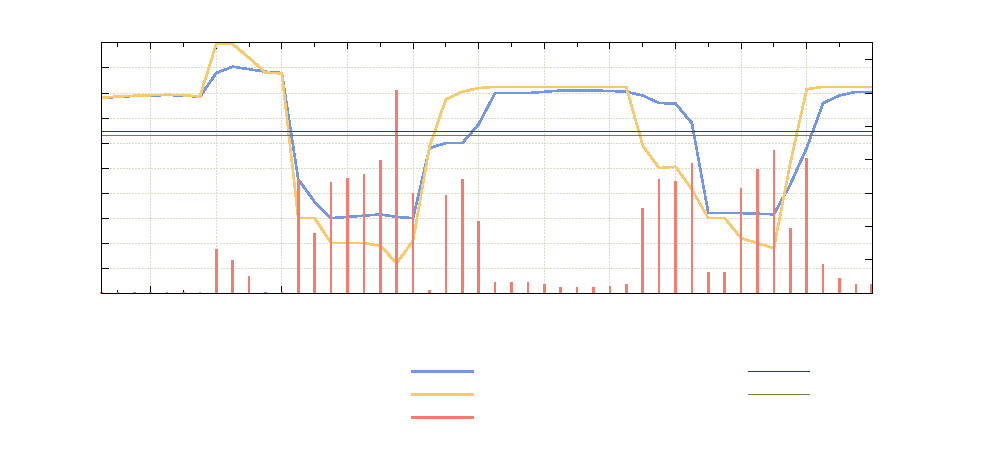
\includegraphics[trim=0 0 0.1cm 0, clip]{Graphs/2/Verification/Verification}}}%
    
    \gplfronttext
  \end{picture}%
\endgroup

 		\caption[Example of simulation error calculation.]{Example of simulation error calculation. Adapted from Marè \cite{Mare2016PhD}}
 		\label{fig:Philipp Difference verify}
 	\end{figure}
 
\subsubsection{Coefficient of correlation and cross correlation}
stuff about correlation blah blah \par more stuff \\
\subsubsection{Mean squared error}
stuff about correlation blah blah \par more stuff \\
 	\subsubsection{Verification in previous simulation studies}
 	Previous studies used verified there simulations through different methods and varying degrees of precision. \\
 	\begin{table}[h]
 		\centering
 		\begin{tabular}{p{5cm}ccr}
 			\hline
 			Study & Year & Verification method & Accepted margin\\
 			\hhline{====}
 			Marais \cite{Marais2012PhD} 						& 2012 & Mean residual \% difference  & Not specified\\
 			Van Niekerk \cite{vanNiekerk2012Value} 				& 2012 &  Mean residual \% difference & 10\% difference \\
 			Bredenkamp \cite{Bredenkamp2013Masters} 			& 2013 & Mean residual \% difference & 10\% difference \\
 			Holman \cite{Holman2014Masters} 					& 2014 & Mean residual \% difference & Not specified  \\
 			Kriel \cite{Marais2012PhD} 							& 2014 &  Mean residual \% difference & 10\% difference \\
 			VanTonder \cite{vanTonder2014PhD}					& 2014 &  Mean residual \% difference & 3\% difference \\
 			Kurnia \textit{et al} \cite{kurnia2014simulation} 	& 2014 & Coefficient of determination ($R^2$) & $>0.95$ \\
 			dominic \cite{dominic2014dynamic}					& 2014 & Mean squared error & $>1.7e^{-3}$	\\
 			Du Plessis \textit{et al}\cite{du2015development} 	& 2015 &  Mean residual \% difference & 7\%  \\
 			Pascoe \cite{Pascoe2016Masters} 					& 2016 &  Mean residual \% difference & 5\% difference \\	
			Peach \cite{Peach2016Masters}						& 2016 &  Mean residual \% difference & Not specified\\
 			Mare \cite{Mare2016PhD} 							& 2016 &  Mean residual \% difference & 5\% difference  \\	
 			Yu-jie-Xu \cite{xu2016modeling}						& 2016 & Mean absolute \% error & 5\%  error\\
 			\hline
 		\end{tabular} 
 		\caption{Simulation verification methods that were implemented in previous studies.}
 		\label{table: Verification studies}
 	\end{table}
\clearpage	
\section{Use of simulation in mining compressed air optimisation}
\subsection{Preamble}
This section will discuss simulation usage in literature to optimise mining compressed air systems.
\subsection{Compressed air simulation models} \label{simplfiedModels}
\subsubsection{Simplified vessel  model}
Before new tools allowed model development for complex mining compressed air simulation models, Marais \cite{Marais2012PhD},\cite{marais2013simplification} created a simplified model to estimate and quantify the performance of potential interventions.  \cite{Marais2012PhD} simplified a mining compressed air system, comparing the network to a compressed air source and a vessel with many leaks. This is illustrated in \cref{fig:Marais vessel model}.
\begin{figure}[h!]
	\centering
	\fbox{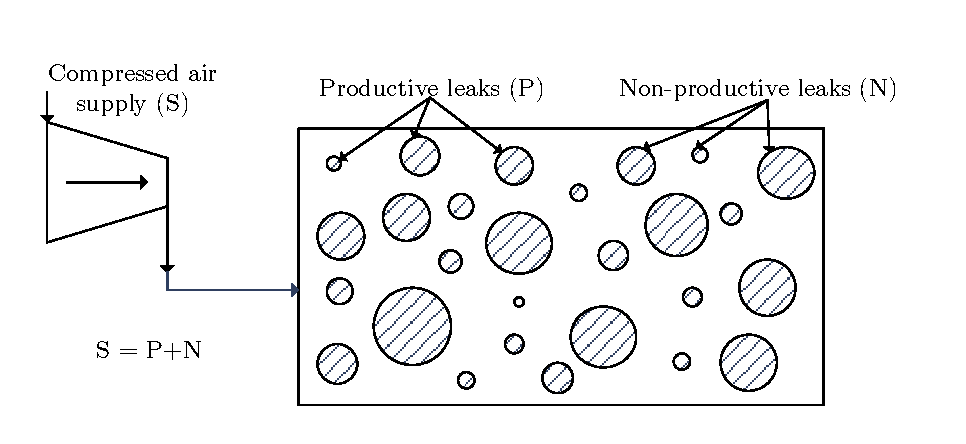
\includegraphics[width=\textwidth]{Images/2/marais/Vessel}}
	\caption[Simplified compressed air netowrk model.]{Simplified compressed air network model. Adapted from Marais \cite{Marais2012PhD}.}
	\label{fig:Marais vessel model}
\end{figure}
\par 
A simplified calculation method was developed to quickly estimate the expected energy savings impact on the system. From this, energy saving estimations rules were developed as shown in \cref{table: Rules of thumb}.  
\par 
The accuracy of this approach is not very high as the specifics of the network are not taken into account. The simplified approach cannot be used for more complex scenarios for example compressor relocation. The study also does not estimate other potential benefits of an intervention such as pressure delivery improvements.
\par 
\begin{table}[h]
	\centering
	\begin{tabular}{p{0.4\textwidth}p{0.05\textwidth}p{0.5\textwidth}}
		\hline
		Intervention && Estimation rule\\
		\hhline{===} 
		Reducing compressor deliver pressure & & $x \%$ pressure reduction  $\propto$ (1.6 to 1.8)$\cdot x\%$ power reduction \newline \\
		Reduce control valve pressure &  &$x \%$ pressure reduction $\propto$  $p\cdot x\%$ power reduction. \newline \newline Where p is the valves percentage flow contribution to the system \newline \\
		Reduction of flow && $x \%$ flow reduction  $\propto x \%$ power reduction \newline\\
		\hline
	\end{tabular} 
	\caption[Summary of energy saving estimation rules]{Summary of energy saving estimation rules\cite{Marais2012PhD}.}
	\label{table: Rules of thumb}
\end{table}

\subsubsection{Simplified system  model}
Kriel \cite{Kriel2014Masters} used simulation to estimate project performance on compressed air. The KYPipe software tool was utilised to develop simulation model for compressed air systems. \cite{Kriel2014Masters} simplified the system for the simulation such that a single compressor and a flow to each level represented the system. The model is shown graphically in \cref{fig:kriel  model}
\begin{figure}[h!]
	\centering
	\fbox{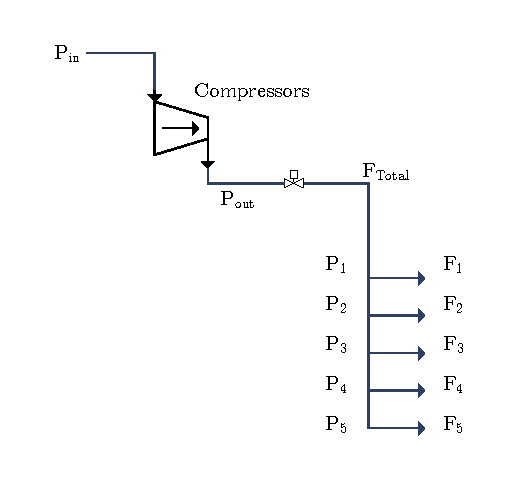
\includegraphics[trim =  -2.5cm 0.5cm -2.5cm 0.5cm ,width=\textwidth]{Images/2/kriel/model}}
	\caption[Simplified system model.]{Simplified system model. Adapted from Kriel \cite{Kriel2014Masters}.}
	\label{fig:kriel  model}
\end{figure}
\par 
Simulation was performed to quantify the savings from underground network interventions. The interventions were deigned to reduce flow to the network. The simulated results varied between 10 and 25\% from the actual performance of the interventions. The simulation procedure in this study could be improved using a more precise model verification method.
\par 

\subsubsection{Compressor relocation}
Bredenkamp \cite{Bredenkamp2013Masters} developed a simulation model to test compressor relocation scenarios. The model, as visualised in \cref{fig: bredenkamp  model}
\begin{figure}[h!]
	\centering
	\fbox{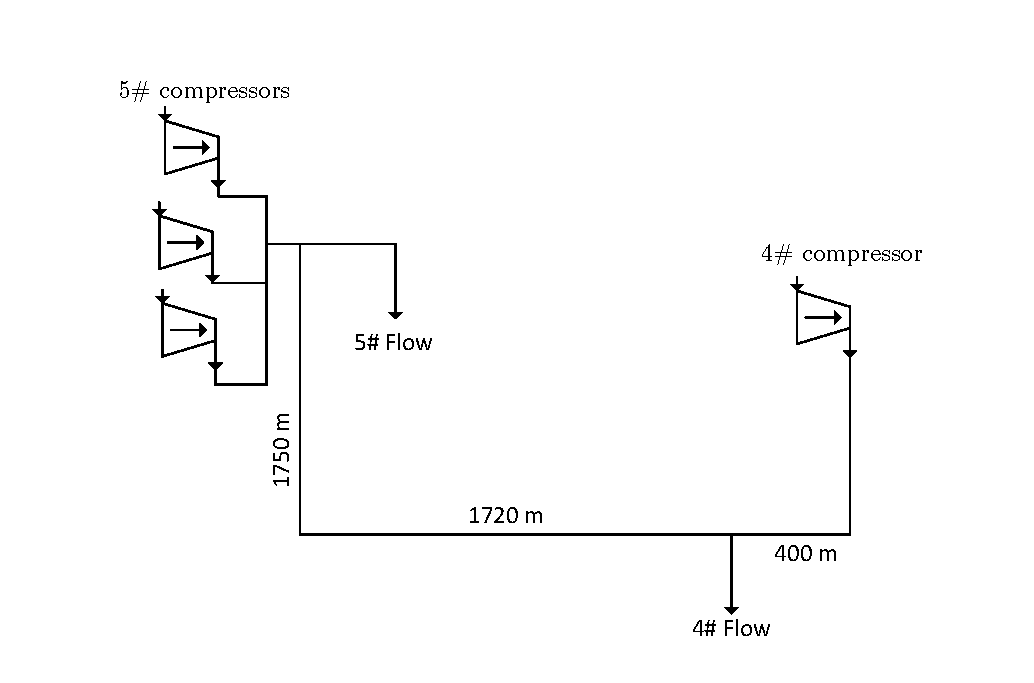
\includegraphics[trim =  -1.2cm 0.5cm -1.2cm 1cm ,width=\textwidth]{Images/2/bredenkamp/model}}
	\caption[Compressor relocation simulation model.]{Compressor relocation simulation model. Adapted from bredenkamp \cite{Bredenkamp2013Masters}.}
	\label{fig: bredenkamp  model}
\end{figure} 
\\
\subsubsection{Compressed air ring}
- Pascoe \\
\begin{figure}[h!]
	\centering
	\fbox{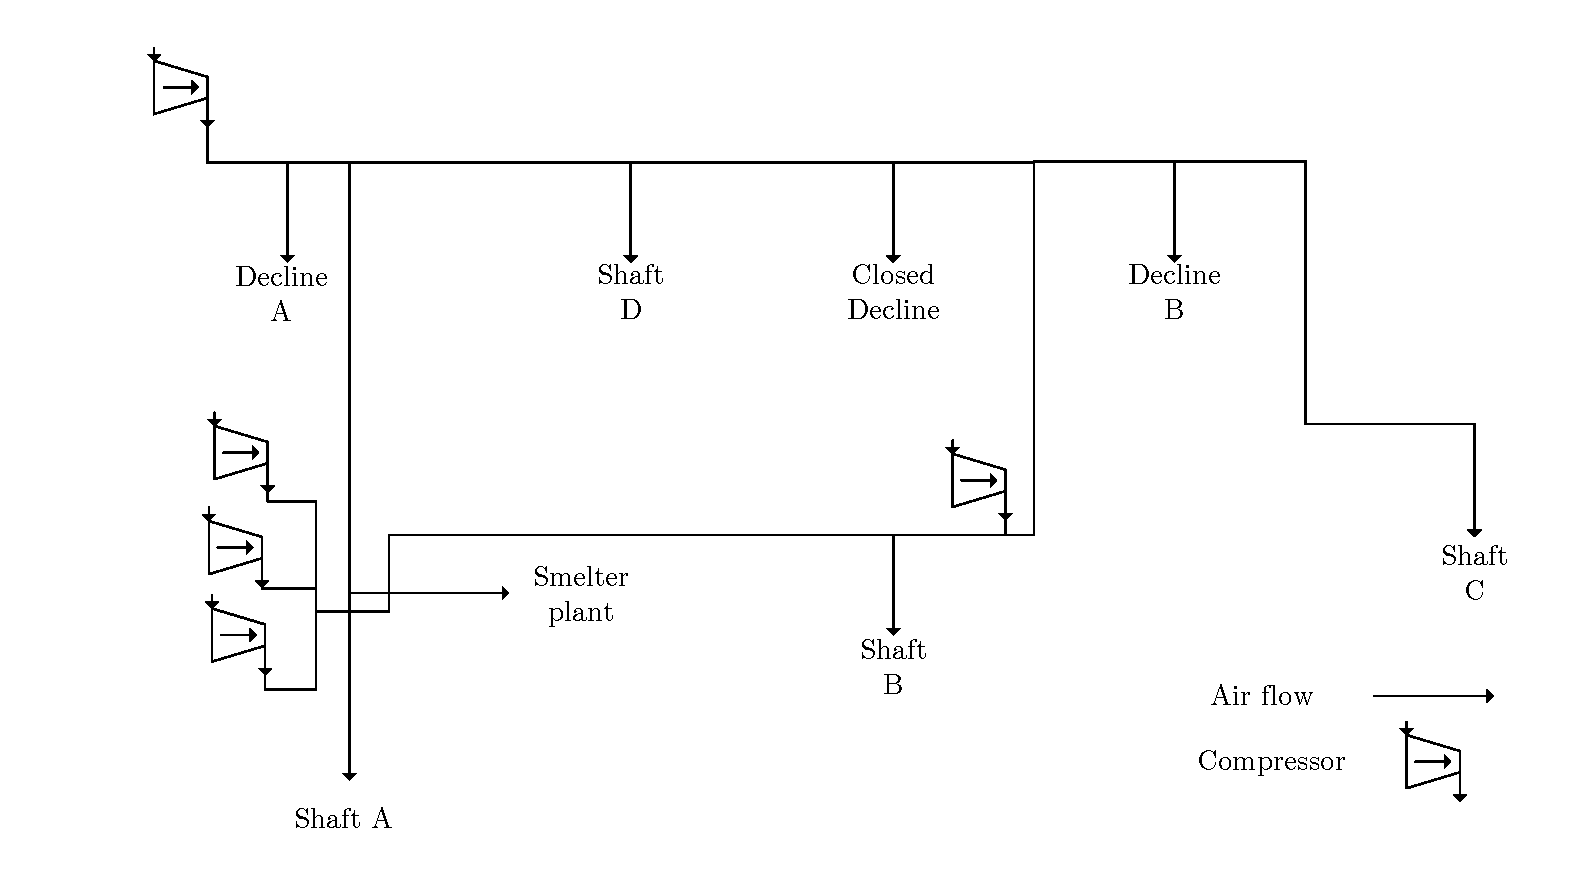
\includegraphics[trim =  -1.5cm 0.5cm -1.5cm 0.5cm ,width=\textwidth]{Images/2/pascoe/model}}
	\caption[Simplified compressed air ring model.]{Simplified compressed air ring model. Adapted from Kriel \cite{Pascoe2016Masters}.}
	\label{fig:kriel  model}
\end{figure}

- Bredenkamp
\\
-Mare et al 

		
		- van Tonder\\
		- De Coning \\-  simulations to investigate the opportunity to optimise the control strategy of a compressed air network by rescheduling the compressors.\\
	\subsection{Summary}
	\label{Shortcomings of previous work}
		\clearpage	
\section{Conclusion}